\documentclass[journal]{IEEEtran}
\usepackage[a5paper, margin=10mm, onecolumn]{geometry}
\usepackage{amsmath,amssymb,amsfonts,amsthm}
\usepackage{gvv-book}
\usepackage{gvv}
\usepackage{hyperref}

\begin{document}

\title{4.3.36}
\author{Puni Aditya - EE25BTECH11046}
\maketitle
\textbf{Question:}\\
The line $\vec{r} = \brak{2\hat{i} - 3\hat{j} - \hat{k}} + \lambda\brak{\hat{i} - \hat{j} + 2\hat{k}}$ lies in the plane $\vec{r} \cdot \brak{3\hat{i} + \hat{j} - \hat{k}} + 2 = 0$.

\textbf{Solution:}\\
Let the line L be $\vec{x}$ = $\vec{a}$ + $\lambda\vec{b}$ and the plane P be $\vec{n}^\top\vec{x}$ = $c$ where
\begin{align*}
    \vec{a} = \myvec{2 \\ -3 \\ -1}, \vec{b} = \myvec{1 \\ -1 \\ 2}, \vec{n} = \myvec{3 \\ 1 \\ -1}, \text{c = -2}
\end{align*}
\begin{align}
    \vec{n}^\top\vec{b} &= \myvec{3 & 1 & -1}\myvec{1 \\ -1 \\ 2} \\
    &= \brak{1}\brak{3}+\brak{-1}\brak{1}+\brak{2}\brak{-1} \\
    &= 3-1-2 \\
    \vec{n}^\top\vec{b} &= 0
\end{align}
$\because \vec{n}^\top\vec{b} = 0$, the line L is parallel to plane P.
\begin{align}
    \vec{n}^\top\vec{a} &= \myvec{3 & 1 & -1}\myvec{2 \\ -3 \\ -1} \\
    &= \brak{2}\brak{3} + \brak{-3}\brak{1} + \brak{-1}\brak{-1} \\
    &= 6-3+1 \\
    &= 4 \neq \text{ c}
\end{align}
$\because \vec{n}^\top\vec{a} \neq c$, the point $\vec{a}$ doesn't line in the plane P. Hence, the line L containing $\vec{a}$ also doesn't lie in the plane. \\
The given statement is \textbf{false}.

\begin{figure}
    \centering
    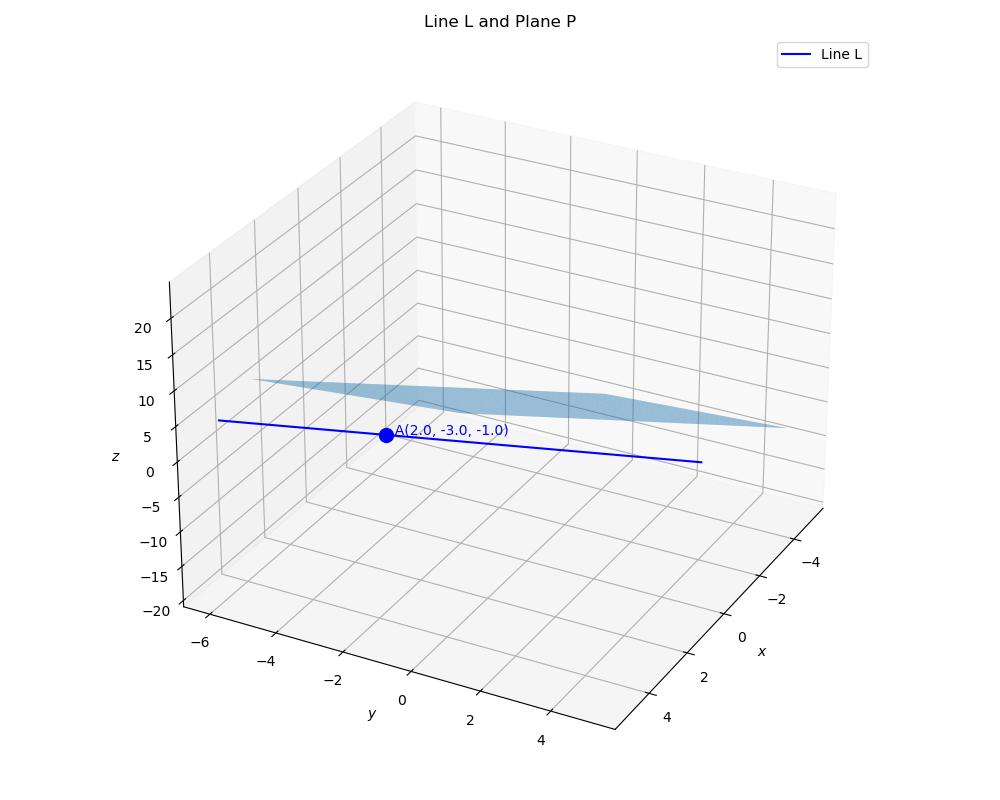
\includegraphics[width=\columnwidth]{figs/plot_c.jpg}
    \caption*{Plot}
    \label{fig:fig}
\end{figure}

\end{document}
